This option allows users to generate synthetic ground motions for a
desired seismic event. When selecting this option, the stochastic
ground loading model is selected from the drop-down menu, as shown
in \autoref{fig:stochastic_loading}. Depending on the model selected,
the user will be asked to enter the parameters describing the seismic
event that the synthetic motion should emulate. In the current
release, users can only select the model proposed by Vlachos et
al. (2018) \cite{vlachos2018predictive}. Additionally, users can
provide a seed for the stochastic motion generation if they desire the
same suite of synthetic motions to be generated.

The backend application that generates the stochastic ground motions
relies on \texttt{smelt}, a modular and extensible C++ library for
generating stochastic time histories for the seismic event. Users
interested in learning more about the implementation and design of
\texttt{smelt} are referred to its
\href{https://github.com/shellshocked2003/Stochastic-Loading-Module}{GitHub repository}.

\begin{figure}[!htbp]
  \centering {
    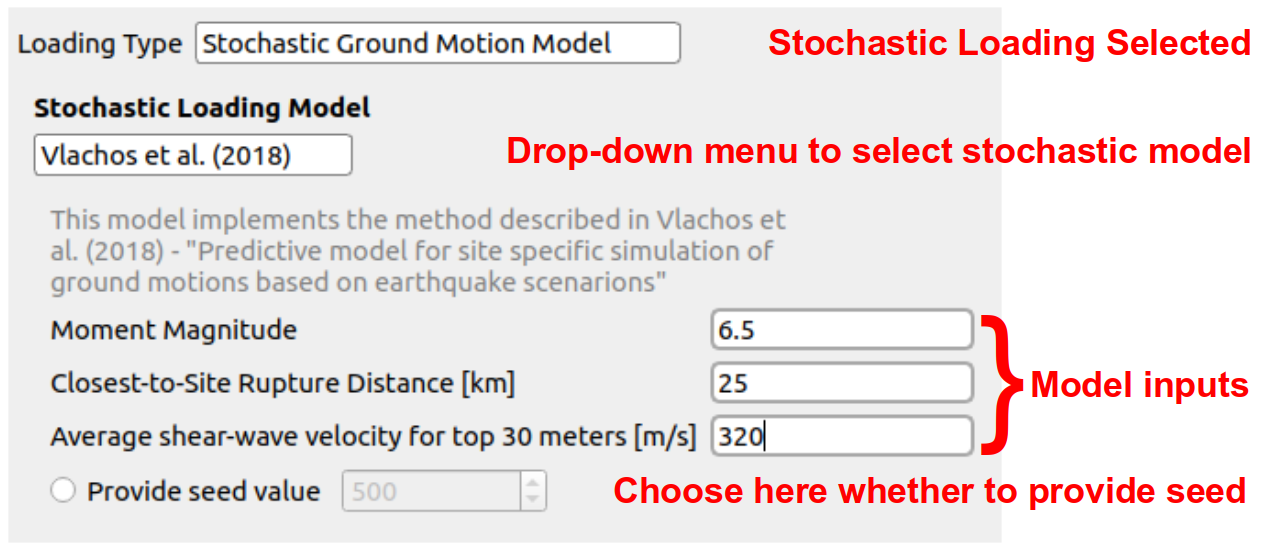
\includegraphics[width=0.8\textwidth]
    {usage/figures/stochastic_loading.png} }
  \caption{Tab appearance when EVT loading type is Stochastic Ground
  Motion Model}
  \label{fig:stochastic_loading}
\end{figure}
